\section{Electromagnetic Waves, Polarization, and Parameters}
\label{intro:electromagnetics_polarization}
A wave can be described as a disturbance that travels through a medium from one location to another location \cite{sanghera2011quantum}. Waves can transfer energy from one point in space to another point in space. Therefore, there are two mechanisms which specify wave properties: The disturbance which defines the wave, and the propagation of the wave. With these, we may classify waves by the following two categories:
\begin{enumerate}
    \item Longitudinal Waves: When the disturbances in a wave are parallel to the wave's propagation direction, the wave is said to be a longitudinal wave. Sound waves, for example, are longitudinal waves because the pressure change occurs parallel to the wave's propagation direction. 
    \item Transverse Waves: When the disturbances in a wave are perpendicular (at right angles) to the wave's propagation direction, the wave is called a transverse wave. Light is an example of a transverse wave, in which energy vibrates in a direction perpendicular to the wave's direction of motion. 
\end{enumerate}
Electromagnetic waves are transverse waves where both the electric and magnetic fields are perpendicular to each other and the direction of wave propagation.

\vspace{-18mm}
%
% Figure: Polarization
%
\begin{figure}[H]
\begin{center}
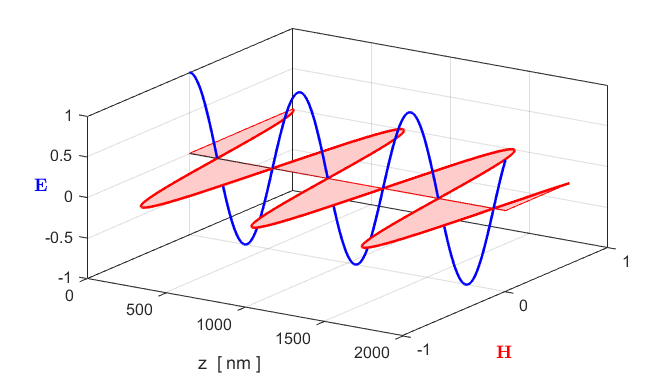
\includegraphics[scale=0.85]{figures/EM_Wave_5.png}
\vspace{0.05 mm}
\caption{A light wave is an electromagnetic wave with an electric and a magnetic component. In our scenario, the electric field $\textbf{E}$ (in blue) oscillates in the vertical direction. The magnetic field $\textbf{H}$ (in red) is at a right angle to the electric field and oscillates in the horizontal direction. Both are perpendicular to the direction of wave propagation ($\textbf{z}$).}
\end{center}
\end{figure}
\vspace{-23mm}

Electromagnetic energy is transmitted in waves 
and an electromagnetic field can propagate along various modes \cite{snyder2012optical,okamoto2021fundamentals,Jackson75}. The three most common modes are \gls{tem}, \gls{te}, and \gls{tm} where
\begin{itemize}
\item TEM Mode: In the Transverse Electric and Magnetic mode, both the electric field and the magnetic field (which, in free space, are always perpendicular to one another) are transverse (at right angles) to the direction of wave propagation (see Figure 3).
\item TE Mode: In the Transverse Electric mode, the electric field is transverse to the direction of propagation while the magnetic field is parallel to the direction of propagation.
\item TM Mode: In the Transverse Magnetic mode, the magnetic field is transverse to the direction of propagation while the electric field is parallel to the direction of propagation.
\end{itemize}
For various reasons the TM mode is of extraordinary importance (e.g., by the classical study of \gls{spr} in Raether \cite{Raether88}) and thus we concentrate our attention on the TM case in Chapters $5$ and $6.$

Throughout this thesis, we are interested in solving electromagnetic problems involving linear, homogeneous, nonmagnetic media. Our strategy, which will be discussed in detail in $\S 1.5$, is to work in the frequency domain by simplifying Maxwell's equations in matter through considering solutions where both the electric and magnetic fields are composed of time--harmonic solutions. These are solutions that have a $e^{-i\omega t}$ time--dependence for a single angular frequency $\omega$. For frequency domain problems, two key material parameters are the permittivity $\epsilon$ and permeability $\mu$. In vacuum, these two quantities are represented by $\epsilon_0$ and $\mu_0$. In addition, we are interested in representing $c$, the speed of light in vacuum, in terms of $c_0$. The index of refraction characterizes the speed of propagation of light in a medium by $n = c_0/c \ge 1$ and allows us to specify the relations
\begin{align*}
c &= \frac{c_0}{n}, &&\text{(Speed in Dielectric Material)}\\
c_0 &= \frac{1}{\sqrt{\epsilon_0\mu_0}}, &&\text{(Speed of Light in Vacuum)}\\
n &= \sqrt{\frac{\epsilon\mu}{\epsilon_0\mu_0}}, &&\text{(Refractive Index)}\\
k_0 &= \frac{\omega}{c_0}, &&\text{(Wavenumber in Vacuum)}\\
k &= nk_0, &&\text{(Wavenumber and Refractive Index)}\\
\lambda &= \frac{2\pi c_0}{\omega}. &&\text{(Wavelength)}
\end{align*}
In many cases, it is enough to specify the quantities $\omega$ and  $n$ so that the remaining dielectric parameters can be found through the permittivity and permeability of the corresponding medium. We will measure the wavelength in microns (where $1 ~\mu \text{m} = 10^{-6}~\text{m}$), as is common in many applications in engineering and photonics. An alternative would be to use nanometers where $1 ~\text{nm} = 10^{-9}~\text{m}$ or $1 ~\mu\text{m} = 10^{3}~\text{nm}$. In vacuum, we have $\epsilon_0 = 8.854187817 \times 10^{-12}~ \text{F/m}~ (\text{farards per meter}), ~\mu_0 = 1.256637061 \times 10^{-6} ~\text{H/m}~ (\text{henry per meter}),$ and the speed of light becomes $c_0 = 299,792,458~\text{m/s}$ \cite{halliday2013fundamentals}. Additionally, we will assume that every material layer is piecewise homogeneous and isotropic, so that $\epsilon$ and $\mu$ are uniform throughout all directions of the medium.